\documentclass{article}

\usepackage[shortlabels]{enumitem}
\usepackage{hyperref}
\usepackage{interval}
\usepackage{listings}
\usepackage{pdflscape}
\usepackage{rotating}
\usepackage{struktex}
\usepackage{tabularx}
\usepackage{tikz}
\usetikzlibrary{positioning}
\usepackage{xcolor}
\definecolor{light-gray}{gray}{.9}

\author{
  Albina Oscherowa (4694823) \\
  Karsten Lehmann (4935758)
}
\date{WiSe 2020}
\title{Hausaufgaben Programmieren - Grundlegende Konzepte (PR10)}

\begin{document}
\maketitle

\newpage

\section*{Aufgabe 3}

\begin{struktogramm}(100, 100)
  \assign{Eingabe : Kredithöhe, Zinssatz}
  \assign{Zinsen := Kredithöhe * Zinssatz / 100}
  \until{Wiederhole bis Rate > Zinsen}
    \assign{Eingabe: rate}
  \untilend
  \assign{Restschuld := Kredithöhe}  
  \while[1]{Solange Restschuld > 0}  
    \assign{Laufzeit := Laufzeit + 1}  
    \assign{Zinsen := Restschuld * Zinssatz / 100}
    \assign{Restschuld := Restschuld + Zinsen - Rate}
    \assign{Zinssumme := Zinssumme + Zinsen}
  \whileend
  \ifthenelse{3}{3} {Restschuld < 0} {Ja}{Nein}
    \assign{Rate := Rate + Restschuld}
    \assign{Ausgabe: Rate}
    \change
  \ifend
  \assign{Ausgabe: Laufzeit, Zinssumme}  
\end{struktogramm}

\newpage
\begin{lstlisting}[language=Fortran, showstringspaces=false]
!! Albina Oscherowa (4694823)
!! Karsten Lehmann (4935758)
PROGRAM bauzins
  IMPLICIT NONE
  REAL :: kredithoehe, laufzeit, rate, restschuld, zinsen, &
       zinssatz, zinssumme
  WRITE (*,*) "Kredithoehe ?"
  READ (*,*) kredithoehe
  WRITE (*,*) "Zinssatz ?"
  READ (*,*) zinssatz

  zinsen = kredithoehe * zinssatz / 100
  
  DO
     WRITE (*,*) "Rate ?"
     READ (*,*) rate

     IF (rate > zinsen) THEN
        EXIT
     END IF
     WRITE (*,*) "Fehler: Die Rate muss groesser als ", &
          zinsen, " sein"
  END DO
  laufzeit = 0
  zinssumme = 0
  restschuld = kredithoehe

  DO WHILE (restschuld > 0)
     laufzeit = laufzeit + 1
     zinsen = restschuld * zinssatz / 100
     restschuld = restschuld + zinsen - rate
     zinssumme = zinssumme + zinsen
  END DO

  IF (restschuld < 0) THEN
     rate = rate + restschuld
     WRITE(*,*) "Letzte Rate :", rate
  END IF

  WRITE(*,*) "Laufzeit: ", laufzeit, " Zinssumme: ", &
       zinssumme
END PROGRAM bauzins
\end{lstlisting}

\section*{Aufgabe 4}

\begin{struktogramm}(100, 100)
  \until{Wiederhole bis n > 0}
    \assign{Eingabe: n}
  \untilend
  
  \assign{Maximum := 0}
  \assign{Minimum := MAX\_INT}
  \assign{Summe := 0}
  \assign{Mittelwert := 0}
  \assign{Maximum := 0}

  \while[1]{Solange i < n}
    \assign{i = i + 1}
    \assign{Eingabe: x}
    \ifthenelse{3}{3} {x $>$ Maximum} {Ja} {Nein}
      \assign{Maximum = x}
      \change
    \ifend
    \ifthenelse{3}{3} {x $<$ Minimum} {Ja} {Nein}
      \assign{Minimum = x}
      \change
    \ifend
    \assign{Summe := Summe + x}
    \assign{Mittelwert := Summe / i}
  \whileend
  \assign{Ausgabe der Ergebnisse}
\end{struktogramm}

\newpage
\begin{lstlisting}[language=Fortran, showstringspaces=false]
!! Albina Oscherowa (4694823)
!! Karsten Lehmann (4935758)
PROGRAM zyklus
  IMPLICIT NONE
  INTEGER :: n, max, min, sum, avg, i, x

  WRITE (*,*) "Dieses Programm gibt das Minimum, das &
       &Maximum, den Durchschnitt"
  WRITE (*,*) "und die Summe einer Endlichen Menge von &
       &ganzen Zahlen aus."
 
  
  DO
     WRITE (*,*) "Maechtigkeit der Menge :"
     READ (*,*) n
     IF (n > 0) THEN
        EXIT
     END IF
  END DO
  
  max = 0
  min = HUGE(min)
  sum = 0
  avg = 0
  i = 0

  DO WHILE (i < n)
     i = i + 1
     WRITE(*,*) "Die ", i, ". Zahl der Menge: "
     READ(*,*) x
     IF (x > max) THEN
        max = x
     END IF
     IF (x < min) THEN
        min = x
     END IF
     sum = sum + x
     avg = sum / i
  END DO

  WRITE(*,*) "Maximum: ", max, " Minimum: ", min, " Summe: ", &
       sum, " Durchschnitt: ", avg
END PROGRAM zyklus
\end{lstlisting}

\section*{Aufgabe 5}

\begin{landscape}
\begin{struktogramm}(200, 100)
  \assign{weiterspielen := wahr}
  \while[1]{solange weiterspielen}
    \assign{Ausgabe der Spielanleitung}
    \until{Solange bis l $<$ r}
      \assign{Eingabe: l, r}
    \untilend
    \assign{i := 0}
    \assign{erraten := falsch}
    \while[1]{solange nicht erraten}
      \assign{z := (l + r) / 2}
      \assign{Ausgabe: z}
      \assign{i := i + 1}
      \until{Solange bis c = "$<$" oder c = "$>$" oder c = "="}
        \assign{Eingabe: c}
      \untilend
      \ifthenelse{2}{4} {c = "="} {Ja} {Nein}
        \assign{erraten := wahr}
        \assign{Ausgabe: Zahl der Versuche i}
        \assign{Ausgabe: Frage nach weiterspielen}
        \until{Solange bis c = "y" oder c = "n"}
          \assign{Eingabe: c}
        \untilend
        \ifthenelse{3}{3} {c = "n"} {Ja} {Nein}
          \assign{Weiterspielen := Falsch}
        \change
        \ifend
        \change
        \ifthenelse {2} {5} {r - l = 0 oder (l = z und c = "$<$") oder (r = z und c = "$>$") } {Ja} {Nein}
          \assign{Ausgabe Logikfehler}
          \assign{Programm beenden}
        \change
          \ifthenelse {2}{2} {(r - z) = 1 und c = "$>$"} {Ja} {Nein}
            \assign{r = l}
          \change
            \ifthenelse {2}{2} {c = "$>$"} {ja} {nein}
              \assign{l = z + 1}
            \change
              \assign{r = z - 1}
            \ifend
          \ifend
        \ifend
      \ifend
    \whileend
  \whileend
\end{struktogramm}
\end{landscape}
\newpage

\begin{lstlisting}[language=Fortran, showstringspaces=false]
!! Albina Oscherowa (4694823)
!! Karsten Lehmann (4935758)
PROGRAM zahlenraten
  IMPLICIT NONE

  CHARACTER :: c
  INTEGER :: i, l, r, z
  LOGICAL :: erraten, weiterspielen

  weiterspielen = .true.

  DO WHILE (weiterspielen .eqv. .true.)
  
     WRITE(*,*) "==========================================="
     WRITE(*,*) " Zahlenraten"
     WRITE(*,*) "==========================================="
     WRITE(*,*) "Der Computer wird Sie nach einer oberen und"
     WRITE(*,*) "unteren Grenze fragen. Denken Sie sich"
     WRITE(*,*) "anschliessend eine Zahl zwischen beiden"
     WRITE(*,*) "Grenzen und der Computer versucht dann diese"
     WRITE(*,*) "Zahl zu erraten. Wenn ihre gedachte Zahl"
     WRITE(*,*) "groesser als die vom Computer erratene Zahl"
     WRITE(*,*) "ist, dann geben Sie '>' ein, ist die Zahl"
     WRITE(*,*) "kleiner '<'. Wenn der Computer richtig"
     WRITE(*,*) "geraten hat, bestaetigen Sie dies mit '='."
     
     WRITE(*,*) "Waehlen Sie die untere Grenze: "
     READ(*,*) l
  
     DO
        WRITE(*,*) "Waehlen Sie die obere Grenze: "
        READ(*,*) r
        
        IF (l < r) THEN
          EXIT
       END IF
    END DO

    i = 0
    erraten = .false.
    
    DO WHILE (erraten .eqv. .false.)
       z = (l + r) / 2
       WRITE(*,*) "Ich rate: ", z
       i = i + 1
       DO
          WRITE(*,*) "Was halten Sie von dem Ergebnis? &
               &(<,>,=)"
          READ(*,*) c
          IF (c == '>' .or. c == '<' .or. c == '=') THEN
             EXIT
          END IF
       END DO
       IF (c == '=') THEN
          erraten = .true.
          WRITE(*,*) "Ich habe folgende Zahl an Versuchen &
               &benoetigt: ", i
          WRITE(*,*) "Moechten Sie noch einmal spielen? &
               &(y,n)"
          DO
             READ(*,*) c
             IF (c == 'y' .or. c == 'n') THEN
                EXIT
             END IF
          END DO
          IF (c == 'n') THEN
             weiterspielen = .false.
          END IF
       ELSE
          IF ((r - l) < 1 &
               .or. (l == z .and. c == "<") &
               .or. (r == z .and. c == ">")) THEN
             WRITE(*,*) "Logikfehler !"
             STOP 1
          ELSE
             IF ((r - z) == 1 .and. c == ">") THEN
                l = r
             ELSE
                IF (c == '>') THEN
                   l = z + 1
                ELSE
                   r = z - 1
                END IF
             END IF
          END IF
       END IF
    END DO
 END DO
END PROGRAM zahlenraten
\end{lstlisting}

\newpage

\textbf{Versuchen Sie, einen mathematischen Zusammenhang zwischen der Anzahl der in Frage kommenden ganzen Zahlen
$n = r - l + 1$ und der maximal erforderlichen Anzahl der Rateversuche $k$ abzuleiten.} \\

In dem Programm wird mit jedem Rateversuch eine Zahl $z \in \mathbb{Z}$ aus der Mitte des Intervalls gewählt.
Falls das Intervall eine ungerade Länge hat, wird $z = \frac{l + r - 1}{2}$ gewählt.
Anschließend wird der Nutzer gefragt, ob die gesuchte Zahl $z$ entspricht, sie größer als $z$ oder kleiner
als $z$ ist.
Falls die gesuchte Zahl größer als $z$ ist, so wird $l = z + 1$ gesetzt und das ganze beginnt von vorn.
Falls die gesuchte zahl kleiner als $z$ ist, wird $r = z - 1$ gesetzt.

Im ungünstigsten Fall (mit der maximalen Anzahl an Rateversuchen) wird diese Halbierung des Intervalls
solange fortgeführt, bis $l = r$ ($n = 1$).
Am Beispiel für das Intervall $\interval{1}{7}$ ist dies hier grafisch veranschaulicht:

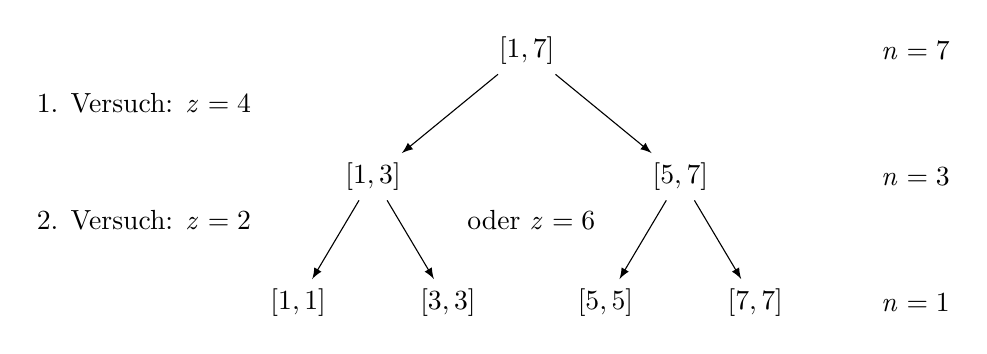
\begin{tikzpicture}
  \node (a) at (0,0) {$\interval{1}{7}$};
  \node[below left = of a] (b1){$\interval{1}{3}$};
  \node[below right = of a] (b2) {$\interval{5}{7}$};
  \node[below left = 1cm and 0cm of b1] (c1) {$\interval{1}{1}$};
  \node[below right= 1cm and 0cm of b1] (c2) {$\interval{3}{3}$};
  \node[below left = 1cm and 0cm of b2] (c3) {$\interval{5}{5}$};
  \node[below right= 1cm and 0cm of b2] (c4) {$\interval{7}{7}$};
  
  \node[right = of c4] (n3) {$n = 1$};
  \node at (b2 -| n3) (n2) {$n = 3$};
  \node at (a -| n3) (n1) {$n = 7$};

  \node[above left = .5cm and 0cm of c1] (k2_1) {2. Versuch: $z = 2$};
  \node[right = 2.5cm of k2_1] (k2_2) {oder $z = 6$};
  \node[above = of k2_1] (k1) {1. Versuch: $z = 4$};
  
  \draw[-latex] (a) -> (b1);
  \draw[-latex] (a) -> (b2);
  \draw[-latex] (b1) -> (c1); 
  \draw[-latex] (b1) -> (c2);
  \draw[-latex] (b2) -> (c3); 
  \draw[-latex] (b2) -> (c4);
\end{tikzpicture}

Daraus schließen wir für den mathematischen Zusammenhang zwischen $n$ und $k$ mit:

\[
  2^{k - 1} \leq n < 2^k
\]

oder auch $k$ ist der auf die nächst kleinere ganze Zahl abgerundete Logarithmus von $n$ zur Basis $2$.

\end{document}